%% NOTICE: ONLY XELATEX WITH EVERYPAGE.STY ENVIRONMENT 
%% CAN COMPILE THIS TEX FILE!
\documentclass[12pt]{article}
\usepackage{xeCJK}
\usepackage{amsmath}
\usepackage{amssymb}
\usepackage{graphicx}
\usepackage{booktabs}
\usepackage{bm}
\setmainfont{FangSong_GB2312}
\title{高级人工智能\footnote{该报告内容均来自中国科学院大学研究生授课教师的高级人工智能
课件,若该报告中相关内容侵犯到了您的版权,请及时联系我们予以删除改正,谢谢! 
联系方式(Email):xiangchao215@mails.ucas.ac.cn}
}
\author{向超\\ \\中国科学院大学}
\date{2016年1月16日}
\begin{document}
\maketitle
\newpage
\renewcommand{\contentsname}{目录}
\renewcommand{\abstractname}{摘要}
\tableofcontents
\newpage
\begin{abstract}
	人工智能(Artificial Intelligence)是当前信息时代最为热门的研究话题,随着人类
计算机硬件和软件技术的飞快提升,人工智能系统层出不穷,各种人工智能硬件和算法在社会的各个领
域被应用,这促使我们细心的整理人工智能相关领域的各个知识系统,对高级人工智能研究领域有一个
较为全面的认识和掌握。为在其他交叉学科领域应用人工智能技术而打下基础。
\end{abstract}
\newpage
\section{不确定性推理}
\subsection{不确定性推理的背景,概念以及结构}
\paragraph{确定性推理和不确定性推理}
\subparagraph{确定性(精确)推理}
逻辑推理方法以数理逻辑为基础,所处理的事实与结论之间存在着确定的因果关系,同时事实也是确定的,
因此得出的结论也是确定的。
\subparagraph{不确定性(非精确)推理}
现实世界中的事物之间的关系是极为复杂的,因此人类的对很多事物以及规律的认知是有限而模糊
不精确的\footnote{例如专家系统中的领域知识就是难以确定的因果关系,它们有些是经验性的知识,
有些甚至是直觉}。
不确定性推理是建立在非经典逻辑基础上的一种推理,是基于不确定性知识的推理\footnote{泛指除
精确推理以外的其他各种推理问题,包括不完备,不精确知识的推理,模糊知识的推理,非单调性推理
等}。非精确推理指的是从不确定性的初始事实或证据出发,通过运用不确定性的知识,最终退出具有
一定程度不确定性却合理或者近乎合理的结论的思维过程。
\subparagraph{人工智能系统的智能}
主要反映在求解不确定性问题的能力上,因此不确定性推理模型是专家系统的一个核心研究问题。
\paragraph{不确定性推理的应用范围}
\subparagraph{所需知识不完备,不精确}
例如医生看病,医生只能得到患者的部分症状,并只能通过专家经
验来做出诊断。
\subparagraph{所需知识描述模糊}
当获取的知识存在描述不清晰不明确的时候,我们需要采用不确定性推理。
\subparagraph{多种原因导致同一结论}
例如多种病因都能导致同一种病症,这个时候只能进行逐个的猜测推断。
\subparagraph{问题的背景知识不足}
面对新的领域,人们对问题本身的了解有可能会被限制,例如Swine Flu, SARS病毒等突然爆发的因素。
\subparagraph{解决方案不唯一}
当解决方案不唯一的时候,人们需要通过某种方法选择主观最优的方案,然而因为问题的解决方案的好坏
因人而异,因此需要一种较为客观的方法从中做出决策。
\paragraph{不确定性推理的重点}
推理方向,推理方法,以及控制策略
\paragraph{不确定性推理的几个基本问题}
\begin{enumerate}
  \item{不确定性的表示}
  \item{不确定性的匹配}
  \item{不确定性的更新算法}
\end{enumerate}
\paragraph{不确定性的表示}
\subparagraph{知识不确定性的表示}
考虑因素:\\
\begin{enumerate}
  \item{问题描述能力}
  \item{推理中不确定性的计算}
\end{enumerate}
表示方法:用数值表示知识确定性程度
\begin{enumerate}
  \item{概率,[0,1],越接近0越假,越接近1越真}
  \item{可信度,[-1,1],小于0为假,大于0表示真}
\end{enumerate}
不确定性程度应该由该知识领域的专家给出。
\subparagraph{证据的不确定性表示}
\begin{enumerate}
  \item{证据通常有两类组成:
    \begin{enumerate}
      \item{初始事实:来源于观察}
      \item{中间结果:因为初始事实具有不确定性,推理过程中所使用的知识也具有不确定性,因此推导过程中产生的中间结果同样带有不确定性}
    \end{enumerate}
  \item{证据的表示:数值形式}
  \item{证据的不确定性表示应与知识的不确定性表示保持一致}
  }
\end{enumerate}
\subparagraph{不确定性的匹配}
\begin{enumerate}
  \item{匹配注意事项:
    \begin{enumerate}
      \item{知识和证据都具有不确定性}
      \item{知识所要求的不确定性程度与证据实际具有的不确定性程度不一定相同}
    \end{enumerate}
  }
  \item{常用的解决方法:
    \begin{enumerate}
      \item{计算相似度,设置阈值。}
      \item{用来计算匹配双方相似程度的算法成为不确定性匹配算法,用来指出相似的限度成为阈值。}
    \end{enumerate}
  }
\end{enumerate}
\subparagraph{不确定性的更新}
两个问题:
\begin{enumerate}
	\item{在推理的每一步中如何利用证据和知识的不确定性更新结论的不确定性?}
	\item{在整个过程中如何把初始证据的不确定性传递给最终结论?}
\end{enumerate}
\subparagraph{不确定性结论的合成}
推理网络中有多个不同知识推出同一结论,且不确定性程度不一样,需要采用算法求解结论的综合不确定性。
\par
\centerline{
	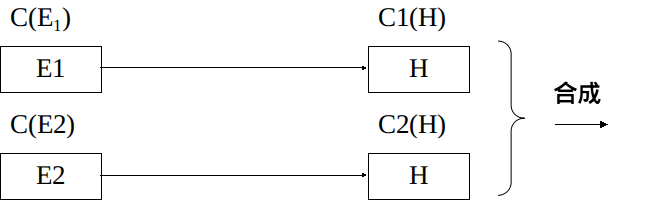
\includegraphics[scale=0.5]{flowchart1.png}
}
\centerline{图1-1 结论合成图}
\par
\subparagraph{不确定性推理的类型}
主要分数值和数值两种方法,在非数值方法中通常采用框架推理或者语义网络推理等,而数值方法多采用基于概率统计的手段进行推理。
\par
\centerline{
	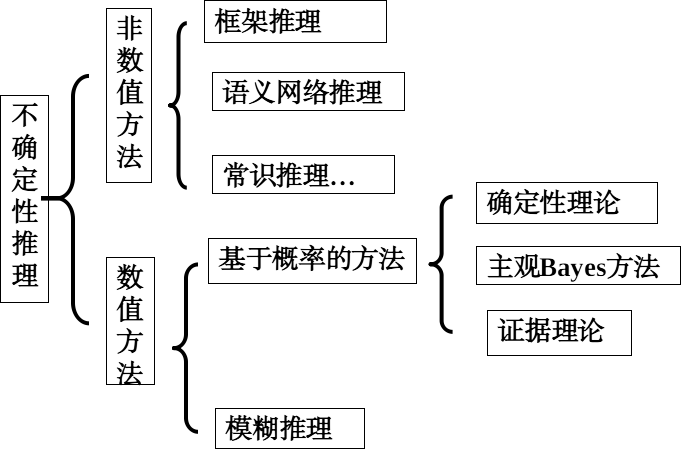
\includegraphics[scale=0.5]{flowchart2.png}
}
\centerline{图1-2 不确定性推理类型结构图}
\par
\subsection{不确定性推理的概率论基础}
\begin{enumerate}
	\item{事件的概率是指事件发生可能性大小}
	\item{条件概率是指事件B发生的条件下考虑条件事件A发生的概率}
	\item{全概率公式与贝叶斯公式}
\end{enumerate}
\paragraph{全概率公式}
设事件$A_1,A_2,...,A_n$满足:
\begin{enumerate}
	\item{任意两个事件都互不相容,即当$i \neq j$时,有
		$$A_i \cap A_j=\emptyset\ (i=1,2,...,n;\ j=1,2,...,n);$$}
	\item{$P(A_i)>0\ (i=1,2,...,n);$}
	\item{全域集合表示为:
		$$D=\bigcup_{i=1}^{n}A_i$$}
\end{enumerate}
则对任何事件B有: 
$$P(B)=\sum_{i=1}^{n}P(A_i)\times P(B|A_i)$$ 
该公式成为全概率公式,它提供一种计算$P(B)$的方法。
\paragraph{贝叶斯(Bayes)公式}
设事件$A_1,A_2,...,A_n$满足上面规定的条件,则对任何事件B都有:
$$P(A_i|B)=\frac{P(A_i)\times P(B|A_i)}{\sum\limits_{j=1}^nP(A_j)\times P(B|A_j)}\ (i=1,2,...,n)$$
该定理称为贝叶斯定理,上面的公式称为贝叶斯公式。\\
其中,$P(A_i)$是事件$A_i$的先验概率,$P(B|A_i)$是事件$A_i$发生条件下事件$B$的条件概率;$P(A_i|B)$是事件$B$发生条件下的事件$A_i$的条件概率。\\
将全概率公式代入贝叶斯公式中,则有:
$$P(A_i|B)=\frac{P(A_i)\times P(B|A_i)}{P(B)}\ (i=1,2,...,n)$$
即 $$P(A_i|B)\times P(B)=P(B|A_i)\times P(A_i)\ (i=1,2,...,n)$$
这是贝叶斯公式的另一种表现形式。从上述公式可以看到,贝叶斯定理给出了通过$P(B|A_i)$求得原概率$P(A_i|B)$的途径。
\subsection{可信度理论}
\paragraph{可信度的概念}
\begin{enumerate}
	\item{可信度是指人们根据以往的经验对某个事物或现象为真的程度的一个判断,或者说是人们对某个事物或现象为真的相信程度\footnote{例如,某同学没来上课,理由是感冒了。这个理由可能为真也可能为假,听到理由的人只能凭借自己所获取的信息判断理由的可信度}。}
	\item{可信度具有一定的主观性,难以把握,单对于某一特定领域,我们一般选择相信领域专家给出的可信度。}
\end{enumerate}
\subsection{CF模型}
\subsubsection{知识不确定性的表示}
\paragraph{在CF(Certainty-Factor)模型中}知识是用产生式规则表示的,其一般形式为:
$$IF\ E\ THEN\ H\ (CF(H,E))$$
其中,$E$是知识的前提条件,而$H$是知识的结论,$CF(H,E)$是知识的可信度。\\
对于上式有以下说明:
\begin{enumerate}
	\item{$E$可以是单一条件,也可以为复合条件\footnote{例如:$E=(E_1\ OR\ E_2)\ AND\ E_3\ AND\ E_4$}。}
	\item{$H$可以是单一结论,可以是多个结论。}
	\item{$CF$是知识的静态强度,$CF(H,E)$的取值区间为$[-1,1]$,当$E$为真时,该值越大,则证据对$H$的支持程度越大。}
\end{enumerate}
例如:$$IF\ 发烧\ AND\ 流鼻涕\ THEN\ 感冒\ (0.8)$$ 表示当某人发烧且流鼻涕时,有80\%的可能性患上了感冒。
\paragraph{CF模型——可信度的定义}
在CF模型中,$CF(H,E)$定义为:
$$CF(H,E)=MB(H,E)-MD(H,E)$$
其中$MB$(Measure Belief)称为信任增长度,$MB(H,E)$定义为:
$$MB(H,E)=\left\{
	\begin{aligned}
		&1,\\
		&\frac{max\{P(H|E),P(H)\}-P(H)}{1-P(H)},\\
	\end{aligned}
	\begin{aligned}
		&若P(H)=1\\
		&否则\\
	\end{aligned}
\right.$$
$MD$(Measure Disbelief)称为不信任增长度,$MB(H,E)$定义为:
$$MD(H,E)=\left\{
	\begin{aligned}
		&1,&&若P(H)=0\\
		&\frac{min\{P(H|E),P(H)\}-P(H)}{-P(H)},&&否则\\
	\end{aligned}
\right.$$
$MB$和$MD$的关系如下:
\begin{enumerate}
	\item{当$MB(H,E)>0$时,有$P(H|E)>P(H)$,即$E$的出现概率增加了$H$的概率}
	\item{当$MD(H,E)>0$时,有$P(H|E)<P(H)$,即$E$的出现概率降低了$H$的概率}
\end{enumerate}
$CF(H,E)$的计算公式:
$$MD(H,E)=\left\{
	\begin{aligned}
		&MB(H,E)=\frac{P(H|E)-P(H)}{1-P(H)},&&若P(H|E)>P(H)\\
		&0,&&若P(H|E)=p(H)\\
		&MD(H,E)=\frac{P(H)-P(H|E)}{P(H)},&&若P(H|E)<P(H)\\
	\end{aligned}
\right.$$
\paragraph{CF模型——可信度的性质}
\begin{enumerate}
	\item{互斥性:对统一证据,它不可能既增加对$H$的信任度,又同时增加对$H$的不信任程度,这说明$MB$和$MD$是互斥的。即
			$$当MB(H,E)>0时,MD(H,E)=0$$
			$$当MD(H,E)>0时,MB(H,E)=0$$}
	\item{值域
				$$0\leq MB(H,E)\leq 1,\ 0\leq MD(H,E)\leq 1,\ -1\leq CF(H,E)\leq 1$$}
	\item{典型值
			\begin{enumerate}
				\item{当$CF(H,E)=1$时,有$P(H|E)=1$,说明,由于$E$所对应的证据的出现使得结论$H$为真。此时,$MB(H,E)=1,\ MD(H,E)=0$。}
				\item{当$CF(H,E)=-1$时,有$P(H|E)=0$,说明,由于$E$所对应的证据的出现使得结论$H$为假,此时,$MB(H,E)=0,\ MD(H,E)=1$。}
				\item{当$CF(H,E)=0$时,有$MB(H,E)=0,\ MD(H,E)=0$。说明$E$所对应的证据的出现无法证实结论$H$,也无法否认结论$H$,没有对结论的可信度产生任何影响。}
			\end{enumerate}
		}
	\item{对$H$信任度的增长等于对$\neg{H}$的不信任度的增长
			\begin{enumerate}
				\item{一个证据对某个假设的成立有利,必然对该假设的不成立不利}
				\item{而且对两者的影响程度相同}
				\item{根据$MD$和$MD$的定义以及概率的性质有
						$$\begin{aligned}
							MD(\neg{H},E)&=\frac{P(\neg{H}|E)-P(\neg{H})}{-P(\neg{H})}\\
							\ &=\frac{(1-P(H|E))-(1-P(H))}{-(1-P(H))}\\
							\ &=\frac{-P(H|E)+P(H)}{-(1-P(H))}\\
							\ &=\frac{-(P(H|E)-P(H))}{-(1-P(H))}\\
							\ &=\frac{P(H|E)-P(H)}{1-P(H)}\\
							\ &=MB(H,E)
						\end{aligned}$$
					}
			\end{enumerate}
		}
\end{enumerate}
根据$CF$的定义结合上述$MB$以及$MD$的互斥性有
$$CF(H,E)+CF(\neg{H},E)=0$$
说明:
\begin{enumerate}
	\item{对$H$的增长度等于对$\neg{H}$的不信任增长度}
	\item{对$H$的可信度与对$\neg{H}$的可信度之和总是为0}
	\item{可信度不同于概率,即
			$$CF(H)+CF(\neg{H})\neq{1}$$
		}
\end{enumerate}
对于同一前提$E$,若支持若干个不同的结论$H_i\ (i=1,2,...,n)$,则
$$\sum_{i=1}^nCF(H_i,E)\leq 1$$
如果发现专家给出的知识存在如下情况
$$CF(H_1,E)=0.7,\ CF(H_2,E)=0.4$$
则因为$0.7+0.4=1.1>0.1$为非法,应该做调整或规范化。\\
在实际应用中,$P(H)$和$P(H|E)$的值都难以获得,因此$CF(H,E)$的值要求由领域专家给出。\\
证据$E$对结论$H$的可信度的影响可以通过$CF(H,E)$的值获知,其原则如下:
\begin{enumerate}
	\item{若由于相应证据的出现将增加结论为真的可信度,则$CF(H,E)>0$,证据的出现越是支持$H$为真,就使$CF(H,E)$的值越大;}
	\item{证据的出现越是支持$H$为假,使$CF(H,E)<0$,$CF(H,E)$的值越小;}
	\item{若证据的出现不影响结论$H$的真假,则使$CF(H,E)=0$;}
\end{enumerate}
\subsubsection{证据不确定性的表示}
证据的不确定性也是用可信度表示的,其取值范围也为$[-1,1]$。且证据的可信度的值由以下方法得到:
\begin{enumerate}
	\item{若$E$为初始证据,其值由用户给出。}
	\item{若$E$伟中间结论,其值可通过计算得到。}
\end{enumerate}
证据$E$的可信度$CF(E)$的取值范围与$CF(H,E)$的取值范围相同,即$-1\leq CF(E)\leq 1$\\
不确定性在这里的含义:
\begin{enumerate}
	\item{$CF(E)=1$,证据$E$肯定为真;}
	\item{$CF(E)=-1$,证据$E$肯定为假;}
	\item{$CF(E)=0$,我们对证据$E$一无所知;}
	\item{$0<CF(E)<1$,证据$E$以某种程度为真;}
	\item{$-1<CF(E)<0$,证据$E$以某种程度为假;}
\end{enumerate}
\subsubsection{证据不确定性的计算}
\paragraph{否定证据不确定性的计算}
$$CF(\neg{E})=-CF(E)$$
\paragraph{组合证据不确定性的计算}
\begin{enumerate}
	\item{合取范式\\当组合证据是多个单一证据的合取时,即$E=E_1\ AND\ E_2\ AND\ ...\ AND\ E_n$时,若已知$CF(E_1),CF(E_2),...,CF(E_n)$,则有
			$$CF(E)=min\{CF(E_1),CF(E2),...,CF(E_n)\}$$
		}
	\item{析取范式\\当组合证据是多个单一证据的析取时,即$E=E_1\ OR\ E_2\ OR\ ...\ OR\ E_n$时,若已知$CF(E_1),CF(E_2),...,CF(E_n)$,则有
			$$CF(E)=max\{CF(E_1),CF(E_2),...,CF(E_n)\}$$
		}
\end{enumerate}
\subsubsection{结论不确定性的更新}
每一次运用不确定性知识,都需要由证据的不确定性和知识的不确定性去计算结论的不确定性。\\
不确定性的更新公式如下
$$CF(H)=CF(H,E)\times{ max\{ 0,CF(E) \} }$$
对于该公式有以下解释
\begin{enumerate}
	\item{若$CF(E)<0$,则$CF(H)=0$,即该模型不考虑证据为假对结论的影响。}
	\item{若$CF(E)=1$,则$CF(H)=CF(H,E)$,则规则强度$CF(H,E)$实际上是在$E$为真时$H$的可信度。}
\end{enumerate}
\subsubsection{结论可信度的合成}
当有多条知识支持同一个结论,这些知识的前提相互独立,且结论的可信度又不想同时,科利用不确定性的合成算法求出结论的综合可信度。\\
设有知识:
$$IF\ E_1\ THEN\ H\ (CF(H,E_1))$$
$$IF\ E_2\ THEN\ H\ (CF(H,E_2))$$
则结论$H$的综合可信度可根据以下步骤计算:
\begin{enumerate}
	\item{分别对每条知识求其结论可信度$CF(H)$:
			$$CF_1(H)=CF(H,E_1)\times max\{0,CF(E_1)\}$$
			$$CF_2(H)=CF(H,E_2)\times max\{0,CF(E_2)\}$$
		}
	\item{采用如下公式计算综合可信度:
			\[ CF(H)=\left\{
			\begin{aligned}
				&CF_1(H)+CF_2(H)-CF_1(H)\times{CF_2(H)}&&
				\begin{split}
					&若CF_1(H)\geq 0\\
					&且CF_2(H)\geq 0\\
				\end{split}\\
				&CF_1(H)+CF_2(H)+CF_1(H)\times{CF_2(H)}&&
				\begin{split}
					&若CF_1(H)<0\\
					&且CF_2(H)<0\\
				\end{split}\\
				&\begin{split}
					&CF_1(H)+CF_2(H)\\
					&或:\frac{CF_1(H)+CF_2(H)}{1-min\{|CF_1(H)|,|CF_2(H)|\}}\\
				\end{split} &&
				\begin{split}
					&若CF_1(H)与\\
					&CF_2(H)异号\\
				\end{split}\\
			\end{aligned}
		\right.\]
		}
\end{enumerate}
\subsubsection{CF模型应用实例}
例如有如下一组知识:
\[
	\begin{split}
		&r_1:\ IF\ E_1\ THEN\ H\ (0.9)\\
		&r_1:\ IF\ E_2\ THEN\ H\ (0.5)\\
		&r_3:\ IF\ E_3\ THEN\ H\ (-0.5)\\
		&r_4:\ IF\ E_4\ AND\ (E_5\ OR\ E_6)\ THEN\ E_1\ (0.8)
	\end{split}
\]
且已知:$CF(E_2)=0.8,CF(E_3)=0.6,CF(E_4)=0.5,CF(E_5)=0.6,CF(E_6)=0.8$,求$CF(H)=?$\\
解:由$r_4$得到:
\[
	\begin{aligned}
		CF(E_1)=&\ 0.8\times max\{0,CF(E_4\ AND\ (E_5\ OR\ E_6))\}\\
		=&\ 0.8\times max\{0,min\{CF(E_4),CF(E_5\ OR\ E_6)\}\}\\
		=&\ 0.8\times max\{0,min\{CF(E_4),max\{CF(E_5),CF(E_6)\}\}\}\\
		=&\ 0.8\times max\{0,min\{0.5,max\{0.6,0.8\}\}\}\\
		=&\ 0.8\times max\{0,min\{0.5,0.8\}\}\\
		=&\ 0.8\times max\{0,0.5\}\\
		=&\ 0.8\times 0.5\\
		=&\ 0.4\\
	\end{aligned}
\]
由$r_1$得到:
\[
	\begin{aligned}
		CF_1(H)=&\ CF(H,E_1)\times max\{0,CF(E_1)\}\\
		=&\ 0.9\times max\{0,0.4\}\\
		=&\ 0.9\times 0.4\\
		=&\ 0.36\\
	\end{aligned}
\]
由$r_2$得到:
\[
	\begin{aligned}
		CF_2(H)=&\ CF(H,E_2)\times max\{0,CF(E_2)\}\\
		=&\ 0.6\times max\{0,0.8\}\\
		=&\ 0.6\times 0.8\\
		=&\ 0.48\\
	\end{aligned}
\]
由$r_3$得到:
\[
	\begin{aligned}
		CF_3(H)=&\ CF(H,E_3)\times max\{0,CF(E_3)\}\\
		=&\ -0.5\times max\{0,0.6\}\\
		=&\ -0.5\times 0.6\\
		=&\ -0.3\\
	\end{aligned}
\]
根据结论不确定性的合成算法,$CF_1(H)$和$CF_2(H)$同号,有:
\[
	\begin{aligned}
		CF_{1,2}(H)=&\ CF_1(H)+CF_2(H)-CF_1(H)\times CF_2(H)\\
		=&\ 0.36+0.48-0.36\times 0.48\\
		=&\ 0.84-0.17\\
		=&\ 0.67\\
	\end{aligned}
\]
由于$CF_{1,2}(H)$和$CF_3(H)$异号,有:
\[
	\begin{aligned}
		CF_{1,2,3}(H)=&\ \frac{CF_{1,2}(H)+CF_3(H)}{1-min\{|CF_{1,2}(H)|,|CF_3(H)|\}}\\
		=&\ \frac{0.67-0.3}{1-min\{0.67,0.3\}}\\
		=&\ \frac{0.37}{0.7}\\
		=&\ 0.53\\
	\end{aligned}
\]
因此综合可信度为:$CF(H)=0.53$\\
\paragraph{CF模型在MYCIN系统中的应用}
MYCIN系统是第一个采用了不确定推理逻辑的专家系统,它是由斯坦福大学开发,用于对细菌感染疾病的
诊断和治疗提供咨询服务,其核心就是CF模型。
\par
\centerline{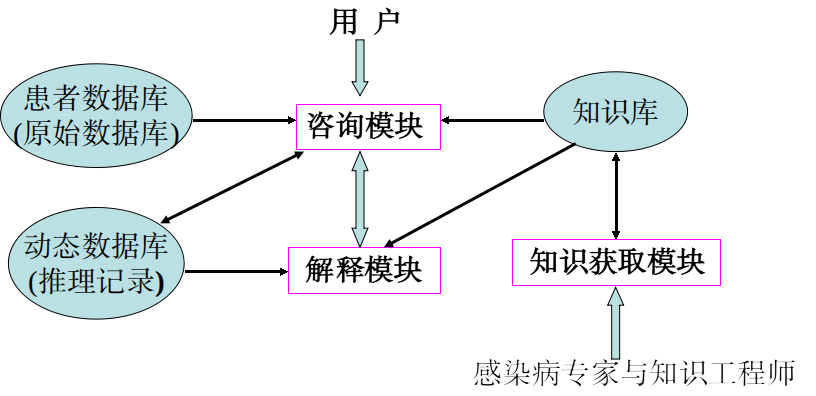
\includegraphics[scale=0.5]{flowchart3.png}}
\centerline{图 1-3 MYCIN系统}
\par
\subsection{证据理论}
证据理论是由德普斯特(A.P.Dempster)首先提出,并由沙佛(G.Shafer)进一步发展起来的用于处理
不确定性的一种理论,因此也被成为DS(Dempster-Shafer)理论。\\
它将概率论中的单点赋值扩展为集合赋值,可以处理由“不知道”所引起的不确定性。因此比主观贝叶斯方法
具有更大的灵活性。\\
在DS理论中,可以分别用信任函数,似然函数以及类概率函数来描述知识的精确信任度,不可驳斥信任度
以及估计信任度。\\
\subsubsection{概率分配函数}
DS理论处理的是集合上的不确定性问题,为此,需要先建立命题与集合之间的一一对应关系,以把命题的
不确定性问题转化为集合的不确定性问题。
\begin{enumerate}
	\item 设$\Omega$为样本空间,且$\Omega$中的每个元素都相互独立,则由$\Omega$所有
子集构成的幂集记为$2^\Omega$。
	\item 当$\Omega$中的元素个数为$N$时,则其幂集$2^\Omega$的元素个数为$2^N$,且其
中每一个元素都对应于一个关于$x$取值情况的命题。
\end{enumerate}
示例如下:\\
设$\Omega=\{红,黄,白\}$,求$\Omega$的幂集$2^\Omega$。\\
解:$\Omega$的幂集可包括如下子集:
\[
	\begin{aligned}
		A_0&=\emptyset\\
		A_1&=\{红\}\\
		A_3&=\{白\}\\
		A_4&=\{红,黄\}\\
		A_5&=\{红,白\}\\
		A_6&=\{黄,白\}\\
		A_7&=\{红,黄,白\}
	\end{aligned}	
\]
其中,$\emptyset$是空集,不难发现子集个数正好是$2^3=8$。\\
概率分配函数定义如下:\\
定义:设函数$m:\ 2^\Omega \to [0,1]$ 满足
\[
	\begin{aligned}
		m(\emptyset)&=0\\
		\sum_{A\subseteq \Omega}m(A)&=1
	\end{aligned}	
\]
则称$m$是$2^\Omega$上的概率分配函数,$m(A)$成为$A$的基本概率数。\\
根据上述概率分配函数的定义,若定义$2^\Omega$上的一个基本函数$m$:
\[
	\begin{split}
	&m(\emptyset,\{红\},\{黄\},\{白\},\{红,黄\},\{红,白\},\{黄,白\},
\{红,黄,白\})\\
	&=(0,0.3,0,0.1,0.2,0.2,0,0.2)\\
	\end{split}
\]
其中,$(0,0.3,0,0.1,0.2,0.2,0,0.2)$分别是幂集$2^\Omega$中各个子集的基本概率数。
显然,$m$满足概率分配函数的定义。\\
理解概率分配函数的概念需要特别注意以下两点:\\
\begin{enumerate}
	\item{概率分配函数的作用是把$\Omega$的任一子集映射到$[0,1]$上的一个数$m(A)$:
		\begin{enumerate}
			\item{当$A\subset\Omega$,且$A$由单个元素组成时,则$m(A)$
			表示对$A$的精确信任度;}
			\item{当$A\subset\Omega,\ A\neq\Omega$,且$A$由多个元素
			组成时,$m(A)$也表示对$A$的精确信任度,但却无法确定该信任度将
			如何分配给$A$的元素;}
			\item{当$A=\Omega$,$m(A)$也无法确定将如何分配信任度。}
		\end{enumerate}
	}
	\item{概率分配函数不是概率,不具有概率的性质。例如\\
		在上例中,$m$符合概率分配函数的定义,但
		\[
			m(\{红\})+m(\{黄\})+m(\{白\})=0.3+0.1=0.4<1
		\]
	因此,概率分配函数不具有概率的性质。
	}
\end{enumerate}
\subsubsection{DS理论——信任函数}
定义:信任函i数$Bel:\ 2^\Omega \to [0,1]$为
\[
	Bel(A) = \sum_{B\subseteq A}m(B)\quad 对所有的 A\subseteq\Omega
\]
其中,$2^\Omega$是$\Omega$的幂集。$Bel$称为下限函数,$Bel(A)$表示对$A$的总的信任度。\\
例如: 
\[
	\begin{aligned}
		Bel(\{红\})&=0.3\\
		Bel(\{红,白\})&=m(\{红\})+m(\{白\})+m(\{红,白\})\\
		&=0.3+0.1+0.2\\
		&=0.6\\
	\end{aligned}
\]
显然,我们很容易得到:
\[
	\begin{aligned}
		Bel(\emptyset)&=m(\emptyset)&=0\\
		Bel(\Omega)&=\sum_{B\subseteq\Omega}m(B)&=1\\
	\end{aligned}
\]
\subsubsection{DS理论——似真度函数}
似真度(Plausibility)函数定义:$Pl:\ 2^\Omega\to[0,1]$为$Pl(A)=1-Bel(\neg A)$,对
所有的$A\subseteq\Omega$成立,其中$\neg A=\Omega-A$。\\
似真度函数又被称为不可驳斥函数或上限函数。由于$Bel(\neg A)$表示对$A$的信任度,
即$A$为假的信任度,因此$Pl(A)$表示对$A$为非假的信任度。\\
例如:\\
\[
	\begin{aligned}
		Pl(\{红\})&=1-Bel(\neg \{红\})\\
		&=1-Bel(\{黄,白\})\\
		&=1-(m\{黄\}+m\{白\}+m\{黄,白\})\\
		&=1-(0+0.1+0)\\
		&=0.9\\
	\end{aligned}
\]
这里的$Pl(\{红\})=0.9$表示“红”为非假的信任度,减去“红”为真的信任度$0.3$,剩下的
$0.9-0.3=0.6$就是知其非假而未能肯定为真的那部分概率了。\\
另一种计算方法如下:\\
\[
	\begin{aligned}
		\sum\limits_{\{红\}\cap{B}\neq\emptyset}m(B)&=
		m(\{红\})+m(\{红,黄\})+m(\{红,白\})+m(\{红,黄,白\})\\
		&=0.3+0.2+0.2+0.2\\
		&=0.9\\
	\end{aligned}
\]
推广到一般情况,可得
\[
	Pl(A)=\sum\limits_{A\cap{B}\neq\emptyset}m(B)
\]
\subsubsection{信任函数与似真度函数的关系}
信任函数与似真度函数之间存在关系:
\[
	Pl(A)\geq Bel(A)
\]
证明如下:
\[
	\begin{aligned}
		\because Bel(A)+Bel(\neg A)&=\sum\limits_{B\subseteq A}m(B)
		+\sum\limits_{C\subseteq\neg A}m(C)\\
		&\leq\sum\limits_{E\subseteq\Omega}m(E)=1\\
		\because Pl(A)-Bel(A)&=1-Bel(\neg A)-Bel(A)\\
		&=1-(Bel(\neg A)+Bel(A))\geq 0\\
		\therefore Pl(A)&\geq Bel(A)
	\end{aligned}
\]
由于$Bel(A)$和$Pl(A)$分别表示$A$为真的信任度和$A$为非假的信任度,因此,可分别
称$Bel(A)$和$Pl(A)$为信任程度的上限和下限。记为:$A[Bel(A),Pl(A)]$。\\
几个经典的值域的含义:\\
\begin{enumerate}
	\item $A[0,1]$:说明对$A$一无所知。即对$A$与$\neg A$都不信任。
	\item $A[0,0]$:说明$A$为假,因为$Bel(A)=0,Bel(\neg A)=1-0=1$。
	\item $A[1,1]$:说明$A$为真,因为$Bel(A)=1,Bel(\neg A)=1-1=0$。
	\item $A[x>0,1]$:说明对$A$为真部分信任。此时$Bel(A)=x>0$
		且$Bel(\neg A)=1-1=0$。
	\item $A[0,0<x<1]$:说明对$\neg A$部分信任,此时$Bel(A)=0$
		且$0<Bel(\neg A)=1-x<1$。
	\item $A[0<x<1,0<y<1]$:说明对$A$与$\neg A$都部分信任。
\end{enumerate}
当证据来源不同时,会得到不同的概率分配函数。
例如:设$\Omega=\{红,黄\}$\\
假设从不同的知识源得到两个不同的概率分配函数:
\[
	\begin{aligned}
		m_1(\emptyset,\{红\},\{黄\},\{红,黄\})&=(0,0.4,0.5,0.1)\\
		m_2(\emptyset,\{红\},\{黄\},\{红,黄\})&=(0,0.6,0.2,0.2)\\
	\end{aligned}
\]
那么我们可以采用德普斯特(Dempster)提出的求正交和的方法来组合这些函数。\\
定义:设同一集合上有来自不同知识源的两个概率分配函数$m_1$和$m_2$,则其
正交和$m=m_1\oplus m_2$满足:
\[
	\begin{aligned}
		m(\emptyset)&=0\\
		m(A)&=K^{-1}\times\sum\limits_{x\cap y=A}m_1(x)\times m_2(y)\\
	\end{aligned}
\]
其中:
\[
	\begin{aligned}
		K&=1-\sum\limits_{x\cap y=\emptyset}m_1(x)\times m_2(y)\\
		 &=\sum\limits_{x\cap y\neq\emptyset}m_1(x)\times m_2(y)\\
	\end{aligned}
\]
如果$K\neq 0$,则正交和也是一个概率分配函数;如果$K=0$,则不存在正交和$m$,
且$m_1$与$m_2$相矛盾。\\
\subsubsection{DS理论的优缺点}
\begin{enumerate}
	\item 优点:能处理由“不知道”所引起的非精确性;样本空间的子集可以是多个
		元素的集合,这样更有利于领域专家在不同层次上进行知识的表示。
	\item 缺点:要求元素(即证据)满足互斥条件,这在实际系统中不易实现;并且,
		需要给出的概率分配数太多,计算比较复杂;证据合成规则没有坚固的理论
		支持,其合理性和有效性还存在较大争议。
\end{enumerate}
\subsubsection{证据理论的推理模型}
\begin{enumerate}
	\item $Bel(A)$和$Pl(A)$分别表示命题$A$的信任度的下限和上限,同时也表示知识
		强度的下限和上限,它们之间的区间表示知识的不确定性强度。
	\item 从信任函数和似真度函数的定义来看,它们都是建立在概率分配函数上的,
		可见不同的概率分配函数得到不同的推理模型。
\end{enumerate}
\subsubsection{一个特殊的概率分配函数}
设$\Omega=\{s_1,s_2,\cdots,s_n\}$,$m$为定义在$2^\Omega$上的概率分配函数,且$m$
满足
\begin{align}
	&m(\{s_i\})\geq 0 \quad  对任何s_i\in\Omega\\
	&\sum\limits_{i=1}^n m(\{s_i\})\leq 1\\
	&m(\Omega)=1-\sum\limits_{i=1}^n m(\{s_i\})\label{eq:omega}\\
	&当A\subset\Omega 且|A|>1或|A|=0时,m(A)=0
\end{align}
其中,$|A|$表示命题$A$所对应的集合中的元素个数。\\
该概率分配函数具有特殊性:
\begin{enumerate}
	\item 只有当子集中的元素个数为1时,其概率分配数才可能大于0;
	\item 当子集中有多个或0个元素且不等于全集时,其概率分配数均为0;
	\item 全集$\Omega$的概率分配数按(\ref{eq:omega})计算。
\end{enumerate}
在这种特殊的概率分配函数下,
定义:对任何命题$A\subseteq\Omega$,其信任函数为
\[
	\begin{aligned}
		Bel(A)&=\sum\limits_{s_i\in A}m(\{s_i\})\\
		Bel(\Omega)&=\sum\limits_{B\subseteq\Omega}m(B)\\
		&=\sum\limits_{i=1}^n m(\{s_i\})+m(\Omega)=1
	\end{aligned}
\]
定义:对任何命题$A\subseteq\Omega$,其似真度函数为
\[
	\begin{aligned}
		Pl(A)&=1-Bel(\neg A)\\
		&=1-\sum\limits_{s_i\in\neg A}m(\{s_i\})\\
		&=1-\left[\sum\limits_{i=1}^n 
		m(\{s_i\})-\sum\limits_{s_i\in A}m(\{s_i\}) \right]\\
		&=1-[1-m(\Omega)-Bel(A)]\\
		&=m(\Omega)+Bel(A)\\
		Pl(\Omega)&=1-Bel(\neg\Omega)\\
		&=1-Bel(\emptyset)=1
	\end{aligned}
\]
对于任意命题$A\subseteq\Omega$和$B\subseteq\Omega$均有:
\[
	Pl(A)-Bel(A)=Pl(B)-Bel(B)=m(\Omega)
\]
它表示对$A$或$B$不知道的程度。
我们再来观察这个特殊的概率分配函数在多源知识下的正交和性质。\\
定义:设$m_1$和$m_2$是$2^\Omega$上的基本概率分配函数,它们的正交和定义为
\[
	m(\{s_i\})=K^{-1}\times[m_1(s_i)\times m_2(s_i)
	+m_1(s_i)\times m_2(\Omega)+m_1(\Omega)\times m_2(s_i)]
\]
其中,
\[
	K=m_1(\Omega)\times m_2(\Omega)+\sum\limits_{i=1}^n 
	[m_1(s_i)\times m_2(s_i)+m_1(s_i)\times m_2(\Omega)
	+m_1(\Omega)\times m_2(s_i)]
\]
\subsection{类概率函数}
定义:设$\Omega$为有限域,对任意命题$A\subseteq\Omega$,命题$A$的类概率函数为
\[
	f(A)=Bel(A)+\frac{|A|}{|\Omega|}\times [Pl(A)-Bel(A)]
\]
其中,$|A|$和$|\Omega|$分别是$A$以及$\Omega$中元素的个数。
\subsubsection{类概率函数的性质}
\begin{enumerate}
	\item $\sum\limits_{i=1}^n f(\{s_i\})=1$
	\item 对任何$A\subseteq\Omega$,有$Bel(A)\leq f(A)\leq Pl(A)$
	\item 对任何$A\subseteq\Omega$,有$f(\neg A)=1-f(A)$
\end{enumerate}
推论
\begin{enumerate}
	\item $f(\emptyset)=0$
	\item $f(\Omega)=1$
	\item 对任何$A\subseteq\Omega$,有$0\leq f(A)\leq 1$
\end{enumerate}
\subsection{知识不确定性的表示}
知识的表现形式:
\[
	IF\ E\ THEN\ H=\{h_1,h_2,\cdots,h_n\}\quad CF={c_1,c_2,\cdots,c_n}
\]
\begin{enumerate}
	\item $E$为前提条件,它既可以是简单条件,也可以是用合取或析取词链接起来的符合条件;
	\item $H$是结论,它用样本空间中的子集表示,$h_1,h_2,\cdots,h_n$是该子集中的元素;
	\item $CF$是可信度因子,用集合形式表示。该集合中的元素$c_1,c_2,\cdots,c_n$用来
	指出$h_1,h_2,\cdots,h_n$的可信度,$c_i$与$h_i$一一对应。$c_i$应满足:
	\[
		\begin{aligned}
			c_i & \geq 0 && i=1,2,\cdots,n\\
			\sum\limits_{i=1}^n c_i & \leq 1\\
		\end{aligned}
	\]
\end{enumerate}
\subsection{证据不确定性的表示}
定义:设$A$是规则条件部分的命题,$E'$是外部输入的证据和已经证实的命题,在证据$E'$的条件下,
命题$A$与证据$E'$的匹配程度为:
\[
	MD(A|E')=\left\{
		\begin{aligned}
			&1 && 如果A中的所有元素都出现在E'中\\
			&0 && 否则
		\end{aligned}
	\right.
\]
定义:条件部分命题$A$的确定性为
\[ CER(A)=MD(A|E')\times f(A) \]
其中$f(A)$为类概率函数。由于$f(A)\in[0,1]$,因此$CER(A)\in [0,1]$。\\
\subsubsection{组合证据的不确定性表示}
当组合证据是多个证据的合取时:
\[
	E=E_1\ AND\ E_2\ AND\ \cdots\ AND\ E_n
\]
则
\[
	CER(E)=min\{CER(E_1),CER(E_2),\cdots,CER(E_n)\}
\]
当组合证据是多个证据的析取时:
\[
	E=E_1\ OR\ E_2\ OR\ \cdots\ OR\ E_n
\]
则
\[
	CER(E)=max\{CER(E_1),CER(E_2),\cdots,CER(E_n)\}
\]
\subsubsection{不确定性的更新}
设有知识$IF\ E\ THEN\ H=\{h_1,h_2,\cdots,h_n\}\quad CF=\{c_1,c_2,\cdots,c_n\}$
则求结论$H$的确定性$CER(H)$的方法如下:
\begin{enumerate}
	\item 求$H$的概率分配函数:
	\[
		\begin{aligned}
			m(\{h_1\},\{h_2\},\cdots,\{h_n\})
			&=(CER(E)\times c_1,CER(E)\times c_2, 
			\cdots, CER(E)\times c_n)\\
			m(\Omega)&=1-\sum\limits_{i=1}^n CER(E)\times c_i
		\end{aligned}
	\]
	当有多条知识支持同一结论$H$时,如有$K$条知识支持同一结论:
	\[
		\begin{aligned}
			&IF\ E\ THEN\ H=\{h_1,h_2,\cdots,h_n\}\quad 
			CF=\{c_{1,1},c_{1,2},\cdots,c_{1,n}\}\\
			&IF\ E\ THEN\ H=\{h_1,h_2,\cdots,h_n\}\quad 
			CF=\{c_{2,1},c_{2,2},\cdots,c_{2,n}\}\\
			&\vdots\\
			&IF\ E\ THEN\ H=\{h_1,h_2,\cdots,h_n\}\quad 
			CF=\{c_{K,1},c_{K,2},\cdots,c_{K,n}\}\\
		\end{aligned}	
	\]
	则按正交和求$CER(H)$,即先求出这$K$条知识的概率分配函数,然后求其正交和:
	\[m=m_1\oplus m_2\oplus\cdots\oplus m_K\]
	这样就能得到最终的符合概率分配函数$m$了。
	\item 求$Bel(H)$,$Pl(H)$,以及$f(H)$:
	\[
		\begin{aligned}
			Bel(H)&=\sum\limits_{i=1}^n m(\{h_i\})\\
			Pl(H)&=1-Bel(\neg H)\\
			f(H)&=Bel(H)+\frac{|H|}{|\Omega|}\times [Pl(H)-Bel(H)]\\
			&=Bel(H)+\frac{|H|}{|\Omega|}\times m(\Omega)
		\end{aligned}
	\]
	\item 求$H$的确定性$CER(H)$:\\
	按公式$CER(H)=MD(H|E')\times f(H)$计算结论$H$的确定性。
	
\end{enumerate}
\subsection{本章总结}
本章主要围绕如何表示证据和知识(规则)的不确定性,并将之推广到多证据复合,多源知识复合的情形,
探究其复合情况下的不确定性的更新方法,并在此过程中为了便于描述不确定性,提出了多个描述和计算
模型,这些模型在实际的专家系统中都的到了应用,为不确定性推理系统提供了较为严谨的理论依据。

\end{document}

